% !TEX root=../main.tex
\chapter{Implementation and Results}
\renewcommand{\baselinestretch}{\mystretch}
\label{chap:results}
% \setlength{\parindent}{0pt}
\PARstart{T}{his} chapter demonstrates the implementation steps based on the theory of previous section. Firstly, the acoustic data of Geoffroy’s spider monkey is clipped and extracted in order to compile the dataset. The baseline model was contributed by Duncan Bulter who studied this relevant project last year. The improvement methods are concentrated on audio denoising, augmentation and hard negative mining. Moreover, a complex deep learning model with the inspiration of VGGNet is proposed and tested. The generalisation error is measured by new test data clips for both models.

\section{Dataset Compiling and Feature Extraction}
\subsection{Data preparation}
The raw audio data are minute-long files in Waveform Audio File Format (WAVE). With the support of software 'Praat', accurate time locations about when the spider monkey call occurs in the minute-long files were recorded in files. However, the raw file is significantly redundant to apply audio data detection. Hence, all of raw files need to be clipped into appropriate length segments. By observing the length of segments of interest, the average length of calls is approximate 1 second and the longest call is 2.1 second. Thus, we selected 3-seconds window to be used for clipping minute-long files. Based on the Python library \texttt{pydub}, the audio file can be manipulated as time series in milliseconds. Firstly, the accurate start and end time of calls were read from Praat-files. Since the duration of calls is smaller than the window length, residual segments can be randomly chose to form 3-seconds clips, which can increase the variety of dataset. Moreover, for guaranteeing the quality of calls, a 20\% margin is restricted between the edge of the window and the edge of call duration. \par
By following these steps, totally 388 positives are clipped from raw data files, corresponding to the statement in Section 1.3. Crump \& Houlahan (2017)~\cite{crump2017designing} stated that the performance of recognizers can be improved by selecting files from different sites as the training dataset. As stated in Section 1.3, seven different locations of audio data are successively named by type 1 to 7. Table \ref{tabel:Positives} depicts that the type-1 \& 6 data occupy a higher percentage of the positive dataset where other types are as complementary.
\begin{table}[h]
\begin{center}
\caption{Number of Positive files in different types}
\label{tabel:Positives}
\begin{tabular}{ | c | c| c | } 
\hline
Type & Num. of Positives & Percentage of whole data (\%) \\ 
\hline
Type-1 (cattappa) & 126 & 32.47 \\ 
Type-2 (osa) & 18 & 4.64 \\ 
Type-3 (shady) & 38 & 9.79 \\ 
Type-4 (other) & 47 & 12.11 \\ 
Type-5 (live-recording) & 25 & 6.44 \\ 
Type-6 (will) & 77 & 22.38 \\ 
Type-7 (tape-recording) & 57 & 14.69 \\ 
\hline
\end{tabular}
\end{center} 
\end{table}\par
As to creating initial negative examples, two different strategies are used. These are:
\begin{itemize}
\item[(1)] randomly sampling from regions in minute-long files which do not contain the spider monkey call, mainly including additive Gaussian noise and environment sounds;
\item[(2)] collecting quantities of other animals' calls in relevant regions, such as howler monkeys, birds and macaws.
\end{itemize}
Additionally, all sampled negatives are 3-seconds length clips without containing the calls of interest. As a result, there are two types of initial negatives dataset that 450 negative files contain clipped environment sounds and noise and another 288 files of other animal calls. Hence, the total number of negatives are approximate twice of positives. As to constructing dataset, the number of negatives is balanced as same as positives. However, the initial negative training data contain a number of white noise called easy negative example, which is effortless for the CNN model to classify. Therefore, the balanced negatives set was firstly appending 288 other animal calls then randomly selecting the remaining number of negatives from noise dataset.
Moreover, the technique of hard-negative-mining was applied as similarly implemented by Mac Aodha et al.~\cite{batdetect18}. Two ways were used for searching for challenging negative examples. Firstly, the initial negative clips were considered as hard examples if they were incorrectly classified with scores over 0.5. Secondly, I successively clipped raw minute-long files into plenty of 3-seconds clips. Then, use the early-stage model to predict all clips and false positive clips are selected as hard examples. \par
\subsection{Data processing}
The original training dataset contains 776 examples with the half number of positives and negatives. The pre-processing methods introduced in Section 3.2 and 3.3 are compared with the original dataset without processing (w/o). These methods are processed based on the time-series signal. As a consequence, a new folder with the processed file were created. Afterwards, the network will be trained by using different files. The number of denoised fold is same as the dataset without processing. Three groups of data were tested, which are denoised method with spectral subsection (SS), the denoised method with MMSE-LSA and hard negative mining based on MMSE-LSA. As to the data augmentation method, I repeat augmented function 5 times to enlarge the number of dataset, resulting in 3880 files in total. For each augmentation, the strategy was random chose from five methods introduced in Section 3.3. Even if the strategies are selected same, the margin and amplitude are still randomly determined. Thus, the diversity and variety of data can be guaranteed.

Before feeding into the CNN network model, the audio data feature were extracted represented as mel-spectrogram. Due to the Python library \texttt{librosa}, the MFCC features were effectively extracted with sample rate of a 48 kHz, 50\% overlap and hamming filter with over 20 ms per frame, resulting in a window size of 1024 samples. Thus, the shape of spectrogram is (128, 282). For evaluating model, the whole dataset was separated into the training set and test set at a ratio of 9:1. 

\section{Baseline Model}
\subsection{Architecture}
Based on the previous work of Duncan, we chose his designed model as the baseline as shown in Fig \ref{fig:baseline}. He defined a CNN model with three convolutional layers with one size $28\times5\times5$ and two $48\times5\times5$. The filter moves one stride without zero paddings. With the activation function of 'Relu', following by MaxPooling layers with size $4\times2$. He added batch normalization layer only after the second convolution layer. Afterwards, flatten layer was applied with 6048 features and feeding into a dense layer with 128 neurons. The prediction score was the output of the sigmoid function in the region of 0$\sim$1. The input and output shapes after each layer are demonstrated in the Appendix \ref{Fig:shapebaseline}. Due to the binary classification problem, the loss function was binary cross-entropy. Moreover, the Adam optimizer with a fixed learning rate $10^{-5}$ was chosen to upgrade weights. Since there are 698 training data, the model was trained in 50 epochs with batch size 16. \par
\begin{figure}[htp]
\centering
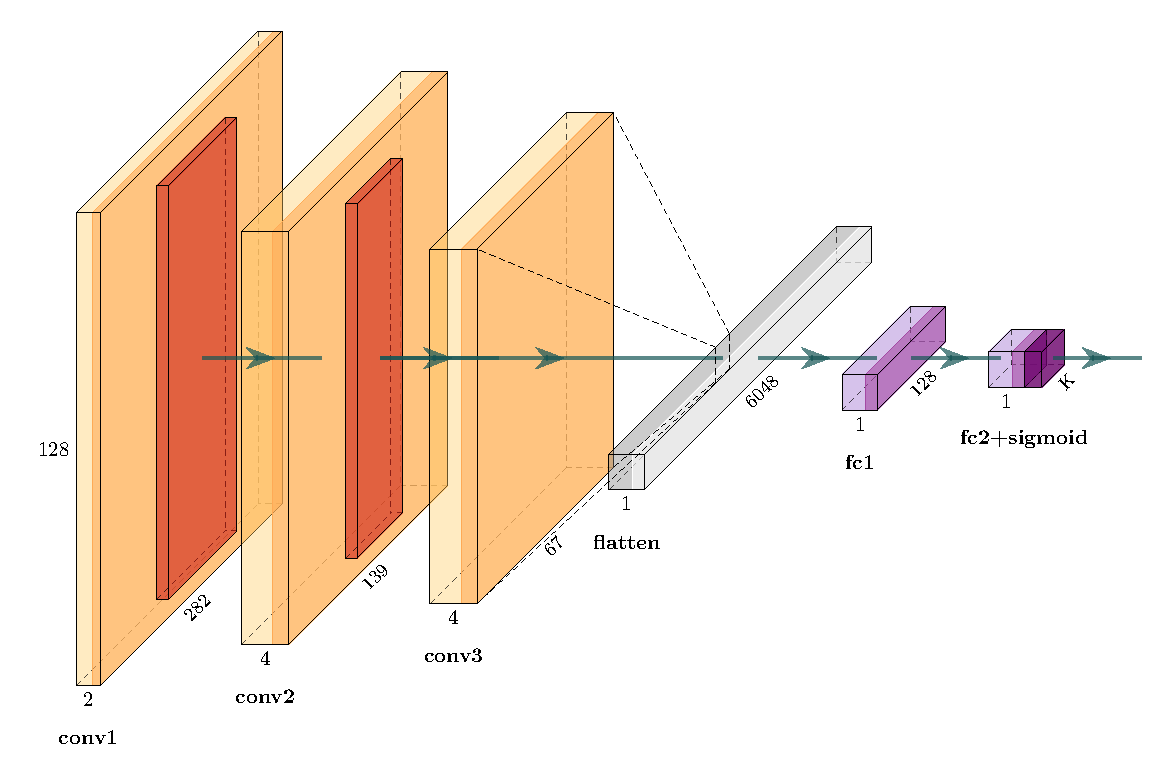
\includegraphics[scale=0.55]{Figs/chap4/baseline.pdf}
\caption{Architecture of the baseline CNN}
\label{fig:baseline}
\end{figure}
Therefore, the baseline model is a relatively shallow convolutional network compared with VGG16 and ResNet. It learns low-level feature to classify the example, which may restrict the performance on detection. The model was first trained with the initial negative training dataset. Then, applied hard negative mining method to train the second time.
\subsection{Results}
\subsection*{Normalization \& Balanced}
The baseline model was separately trained to demonstrate the effects of balanced and normalised data. The strategy of the balanced dataset is introduced in Section 4.1.1 and the number of unbalanced dataset consists of 388 positives calls and 738 negatives. The normalisation was applied both on time-series signal before extraction and on the logarithmic magnitude mel-spectrogram. Table \ref{tab:balanc} shows the metrics scores of these strategies.\par
\begin{table}[htp]
    \centering
    \caption{Scores of balanced and unbalanced dataset with/without normalization}
    \label{tab:balanc}
    \resizebox{0.9\textwidth}{!} & 60.87 & 60.26  & 65.38  & \textbf{66.99}   \\ \hline
    \textbf{Precision\%}      & 57.84                & 52.04      & 65.32    & \textbf{67.75}      \\ \hline
    \textbf{Recall\%}   & 66.18        & 54.89        & \textbf{67.07}      & 63.13   \\ \hline
    \textbf{F1\%}          & 61.43                     & 50.10    & \textbf{66.1}     & 64.89     \\ \hline
    \end{tabular}}
\end{table}
For the dataset without normalisation, the balanced data has a relatively low precision, which means that plenty of negatives are classified as false positive. The unbalanced dataset fails to improve the performance without normalisation, presenting in nearly 50\% precision, recall and F1 score. As to the normalised dataset, both balanced and unbalanced dataset obtain over 60\% scores. The balanced one attains enhanced recall and F1 score, while the accuracy and precision of unbalanced model are a little better.

Normalisation is a significant part before training. Due to the audio data were collected in the volatile tropical environment at different locations, the within-class variance for both positives and negatives are significantly large. Hence, without normalisation, the model will be disturbed by the non-uniform data distribution during training. As shown in Table \ref{tab:balanc}, the accuracy and F1 score are improved 5\% for the balanced dataset. The precision has significant improved and slightly increase in recall since all data were normalized to the range $0\sim1$. As to unbalanced dataset, normalisation can reduce the diversity of data distribution to a large extent, presenting in a distinct increment of all metric scores. Therefore, the unbalanced normalised dataset achieves the highlighted accuracy and precision. However, the recall and F1 scores still fall down. In general, training with unbalanced dataset seems less helpful for performance. The reason may be that, due to the unbalanced number of data, the model tends to concentrate more on negatives, which causes the decline of recall and F1 score. As a result, training with normalised unbalanced dataset achieves a relatively higher accuracy and precision with 66.99\% and 67.75\% respectively. Recall and F1 score are outstanding of the balanced normalised dataset. Observing metric scores in overall, the normalised balanced data strategy was determined to be used.

\subsection*{Pre-processed methods}
As to evaluating the data processing methods, three groups of results are shown in Table \ref{tabel:base  dataset} as control groups on performance. In order to control variables, all dataset are balanced and normalised before training, as discussed in previous section. It took nearly 40 minutes to train the model with 698 data and more than 1.5 hours for augmentation on CPU.
\begin{table}[htp]
\centering
\caption{Metrics scores of baseline model with data processing methods}
\label{tabel:base dataset}
\resizebox{0.9\textwidth}{!} & \textbf{Precision\%} & \textbf{Recall\%} & \textbf{F1 score\%} \\ \hline
\textbf{Orig: Initial} & 65.38 & 65.32 & 67.07 & 66.1 \\
\textbf{Orig: hnm} & 69.23 & 82.34 & 61.65 & 69.85 \\ \hline
\textbf{SS: Initial} & 73.08 & 76.17 & 58.89 & 65.86 \\
\textbf{LSA: Initial} & 76.92 & \textbf{84.10} & \textbf{75.72} & \textbf{78.79} \\
\textbf{LSA: hnm} & 74.36 & 82.05 & 68.72 & 73.41 \\ \hline
\textbf{Aug: Initial} & 76.29 & 78.27 & 71.72 & 73.53 \\
\textbf{Aug: hnm} & \textbf{77.84} & 83.72 & 68.89 & 74.54 \\ \hline
\end{tabular}}
\end{table}
\begin{figure}[!htb]
     \begin{subfigure}[b]{0.5\linewidth}
         \centering
          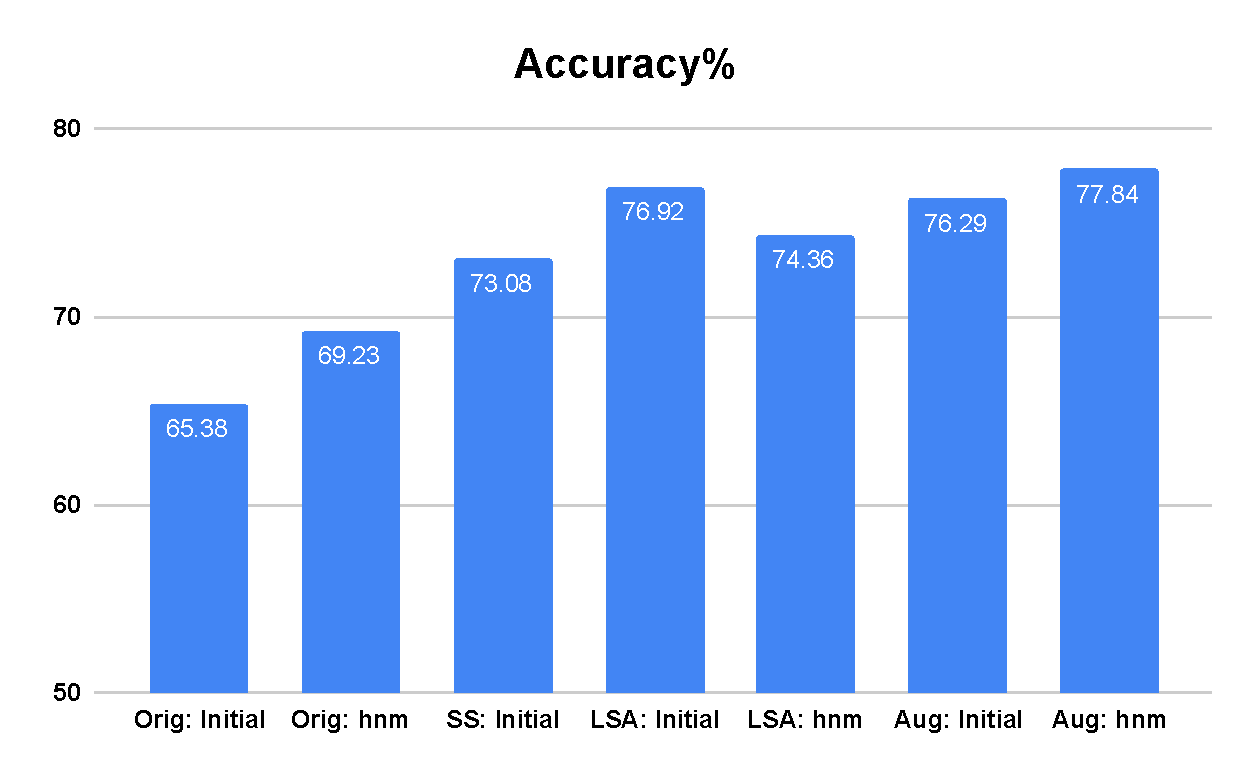
\includegraphics[scale=0.35]{Figs/chap4/baseacc.pdf}
          \caption{Accuracy}
     \end{subfigure}
     ~
     \begin{subfigure}[b]{0.5\linewidth}
         \centering
          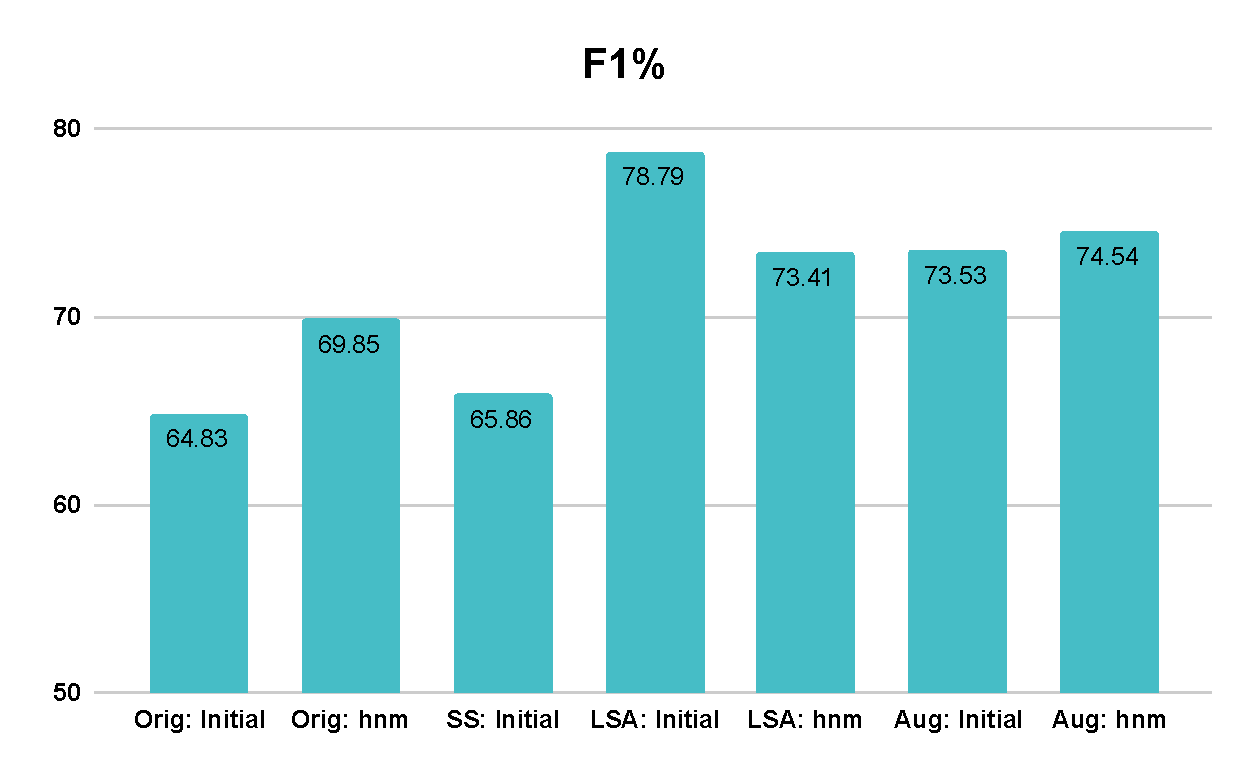
\includegraphics[scale=0.35]{Figs/chap4/basef.pdf}
          \caption{F1 score}
     \end{subfigure}
     \\
     \begin{subfigure}[b]{0.5\linewidth}
         \centering
          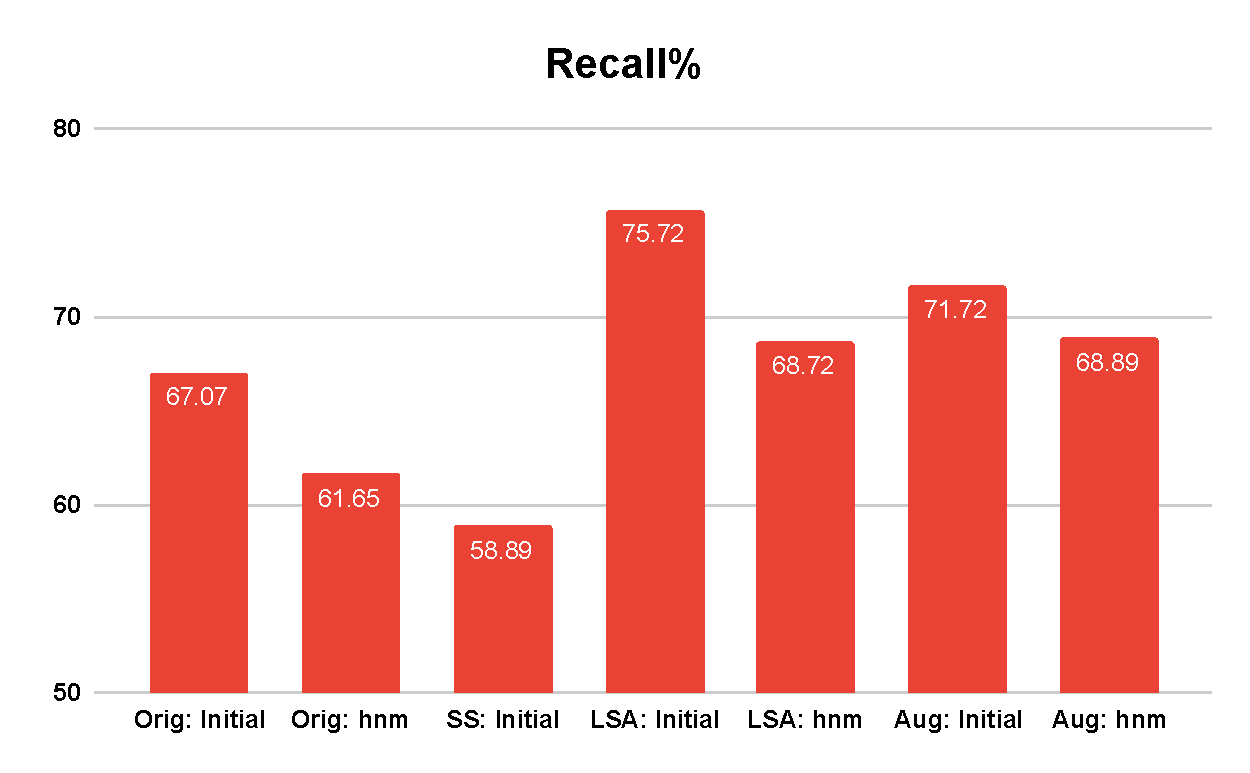
\includegraphics[scale=0.35]{Figs/chap4/baserec.pdf}
          \caption{Recall}
     \end{subfigure}
     \begin{subfigure}[b]{0.5\linewidth}
         \centering
          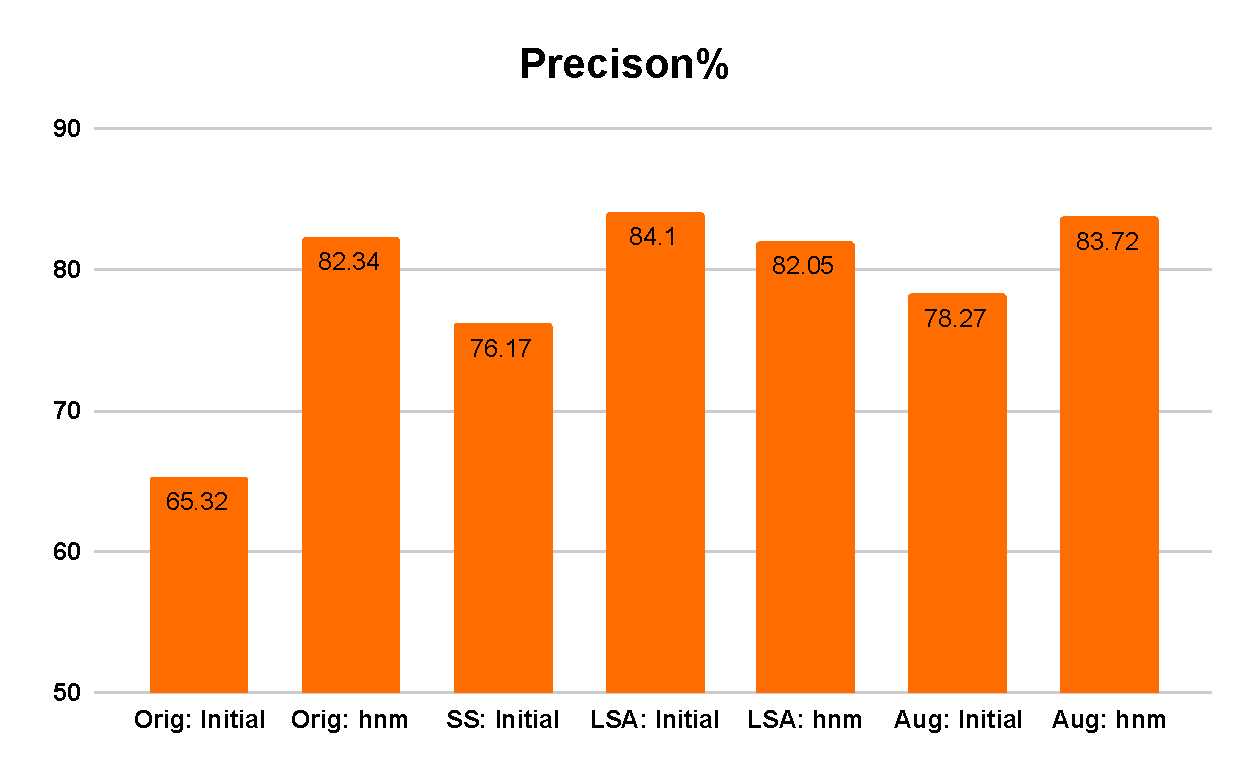
\includegraphics[scale=0.35]{Figs/chap4/basepre.pdf}
          \caption{Precision}
     \end{subfigure}
  \caption{Histograms of baseline model: comparing 7 different strategies in accuracy, F1, recall and precision}
  \label{Fig:hist}
\end{figure}
\begin{itemize}[leftmargin=*]
    \item \textbf{Original data}\\
    The results for the initial dataset without processing are same as the third column of Table \ref{tab:balanc}. After applying hard negative mining method, all metric scores are improved instead of recall. The precision significantly rises up from 65.32\% to 82.34\%, while accuracy and F1 score grow by approximate 4\%. The hard negative mining results in a reduction of recall. The possible reason is that selecting hard negatives will reduce the average distance between positives and hard negatives. Hence, the classifier can accurately recognize the hard negative with increasing precision. However, a number of hard positives (which are close to hard negatives) are affected by easy positive examples, leading to difficult classification.
    \item \textbf{Noise reduction}\\
    Since only positive calls are concerned in this project, both of spectral subtraction (SS) and MMSE-LSA denoising methods are only applied to the positive dataset before training. As shown in results, the noise reduction has the ability to improve the general performance, comparing with the dataset without processing. Specifically, the spectral subtraction retains the performance of recall to a large extent, although the accuracy and precision are improved. As introduced in Section 3.2.1, parts of the information in the region of interest were eliminated during processing, which has significantly impact on classification on positives. Thanks to its simple algorithm, SS denoising method is a time-saving process. \par
    As to MMSE-LSA approach, the results proved its effectiveness and feasibility on species detection. The model achieves impressively scores on initial dataset over whole processing strategies. Even if the accuracy is slightly lower than augmentation, the results still demonstrate its performance. However, using hard negative mining to train this model second time introduces an overall decline in performance, especial in the recall. This is same as the dataset without processing. Thus, the hard negative mining has less contribution to performance. Because we only utilized noise reduction on positive data, which affects the representation distance between positives and negatives to a large extent. Thus, hard negative seems incapable to further improve the performance. Hence, the trained model with denoised dataset may suffer from generalisation error, which is unable to provide accurate predictions on generalised tasks.
    \item \textbf{Augmentation}\\
    The model trained with the augmented dataset can reduce the generalisation error due to the variety and diversity of augmentation. The metric scores goes up over 70\% compared with the original dataset. However, the baseline model shows unremarkable results of augmentation, comparing with denoised dataset. Only accuracy of hard negative mining exceeds other strategies with 77.84\%. The baseline model is not quite deep, which can only learn relative low-level features to classify. MMSE-LSA significant remove the redundant information of mel-spectrogram. This allows the baseline model to put more attention to learn the contributive features. Although augmented dataset increases the generalisation of the model, it is still arduous for the baseline model to learn crucial features. As a result, model trained with denoised dataset obtains higher scores than augmentation. 
\end{itemize} 

In order to determine the optimal strategy for baseline model, the results are presented in visible way to compare, as shown in Fig \ref{Fig:hist}. All of the data processing methods have improved accuracy and precision with over 70\%. The accuracy has an nearly upward tendency with varying processing method. The first trained model with MMSE-LSA (LSA: Initial) and second trained model with augmentation (Aug: hnm) attain increased accuracy. The model of MMSE-LSA with initial dataset has outstanding performance on F1 and recall. However, the spectral subtraction performs underwhelming due to its recall and F1 score.
\section{VGG-based Model}
\begin{figure}[!htb]
\centering
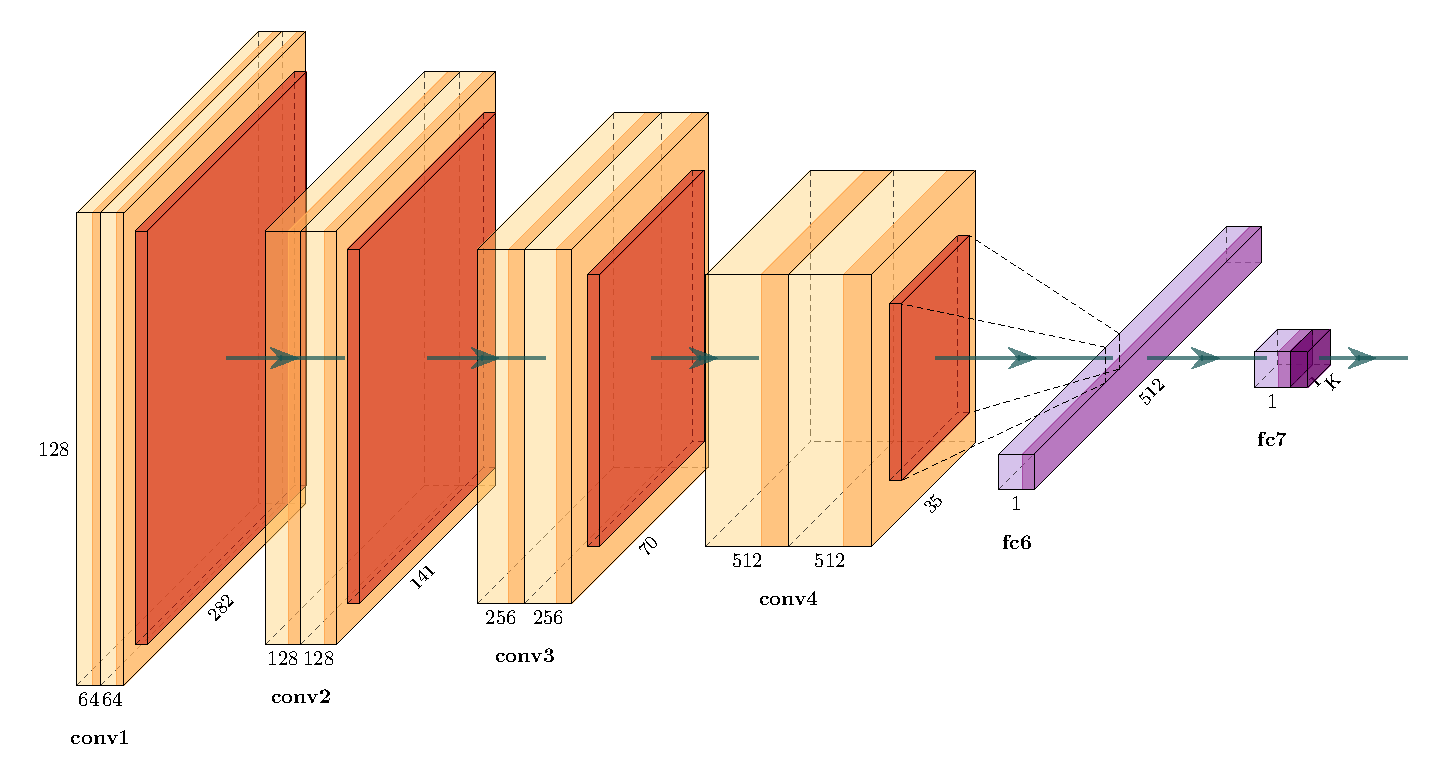
\includegraphics[scale=0.55]{Figs/chap4/vgg16.pdf}
\caption{Architecture of VGG-based CNN}
\label{fig:vgg}
\end{figure}
\subsection{Architecture}
Since the baseline model only contains three convolutional layers, low-level features were learned by this model, resulting in limited ability of detection. With the inspiration of the architecture of VGG16 \cite{simonyan2014very}, I proposed a similar network named VGG-based. Comparing with VGG16, this model is not very deep with only ten weighted layers (6 convolutional layers and 2 FC layers). The visulisation of VGG-based architecture is illustrated in Fig \ref{fig:vgg}. The $5\times5$ size filter of baseline model were replaced by two successive $3\times3$ filters, following with the maxpooling layer in size $2\times2$. For each hierarchical layers, the number of filters in convolutional layer are double, aiming to learn high-level features. Moreover, the batch normalisation layer are added after convolution. The dropout layer with ratio 0.5 was used between FC layers to prevent overfitting. Table \ref{tab:struc} compares the structure depth of baseline and VGG-based model. As a result, $4.03\times10^{7}$ parameters need to be learned, 50 times larger than baseline model. In addition, the hyperparameters for VGG-based model are same as the baseline.
\begin{table}[htp]
\centering
\caption{Comparing depth of models}
\label{tab:struc}
\resizebox{0.6\textwidth}{!}{%
\begin{tabular}{c|c|c}
\hline
 & Baseline & VGG-based \\ \hline
\multirow{3}{*}{1} & conv(24,5,5) & conv(64,3,3) \\
 &  & conv(64,3,3) \\
 & maxpooling(4,2) & maxpooling(2,2) \\ \hline
\multirow{3}{*}{2} & conv(48,5,5) & conv(128,3,3) \\
 &  & conv(128,3,3) \\
 & maxpooling(4,2) & maxpooling(2,2) \\ \hline
\multirow{3}{*}{3} & conv(48,5,5) & conv(256,3,3) \\
 &  & conv(256,3,3) \\
 &  & maxpooling(2,2) \\ \hline
\multirow{3}{*}{4} &  & conv(512,3,3) \\
 &  & conv(512,3,3) \\
 &  & maxpooling(2,2) \\ \hline
\multirow{2}{*}{FC} & FC128 & FC512 \\
 & FC1 & FC1 \\ \hline
 & \multicolumn{2}{c}{sigmoid} \\ \hline
\#param & $8.61\times10^{5}$ & $403\times10^{5}$ \\ \hline
\end{tabular}%
}
\end{table}
\subsection{Results}
\begin{table}[htp]
\centering
\caption{Metrics score of Complex VGG-like model with three dataset strategies}
\label{tabel:VGG dataset}
\resizebox{0.9\textwidth}{!} & \textbf{Precision\%}  & \textbf{Recall\%}& \textbf{F1 score\%}\\
\hline
\textbf{Orig: Initial}& 71.79 & 71.45 & 73.54 & 72.05 \\
\textbf{Orig: hnm} & 70.51 & 75.28 &  76.13 & 75.13\\ 
\hline
\textbf{LSA: Initial} & 76.92 & 81.72 &  77.96 & 79.64\\ 
\textbf{LSA: hnm}& 73.08 & 72.96 &  73.84 & 73.22\\
\hline
\textbf{Aug: Initial}  & 84.54 & 84.59 & \textbf{85.94} & \textbf{84.27}\\
\textbf{Aug: hnm}& \textbf{85.05} & \textbf{89.74} &79.56 & 83.32\\ 
\hline
\end{tabular}}
\end{table}
The VGG-based model was trained in the same way as discussed in baseline model. Due to the increased depth, the VGG-based model effectively improved the performance. Table \ref{tabel:VGG dataset} illustrated the metric scores of these methods. Note that the spectral subtraction did not test in VGG-based model since its underwhelming performance. Training VGG-based model took more than 10-fold time on CPU. Thus, all training works were completed on Amazon Web Services (AWS) by GPUs, with approximate 15 minutes on small dataset and 50 minutes on augmentation. 
\begin{itemize}[leftmargin=*]
    \item \textbf{Original data}\\
     By learning high-level features, the VGG-based model with initial dataset without processing can attain scores over 70\%. After applying hard negative mining, the performance is further improved by approximate 3\% in precision, recall and F1 score. Comparing with the same dataset of baseline model, only precision has impressive scores in 82.34\%. Nevertheless, the training work for VGG-based model is significant time-cost than baseline model.
    \item \textbf{Noise reduction}\\
    The noise reduction method provides less contributive improvement of VGG-based model. Metric scores are approximately similar to the baseline of denoising dataset. Because the MMSE-LSA removed most of the background noise, high-level features can not be further learned by increasing depth of architecture. Additionally, applying hard negative mining on denoised data causes a decreasing performance on VGG-based model as well. It indicates that training with denoised dataset will introduce bias for classification. The model only can detect the positive call without noise, leading to limited robust on noise.
    \item \textbf{Augmentation}\\
    Training with augmentation dataset achieves prominent results for VGG-based model. All scores reach or exceed 80\%, presenting in enhanced accuracy and precision about 85.05\% and 89.74\%with hnm dataset. Nevertheless, the hard negative mining still introduces a decline in recall about 6\%, resulting in relatively decreased F1 score. With contributions of augmentation, the VGG-based model can learn various and diverse data in high-level representation. On the contrary, the shallow network is incapable to effectively classified with low-level features, even if data were augmented in increased variety and diversity.
\end{itemize}
As illustrated in Fig \ref{Fig:histvgg}, the VGG-based model after augmentation significantly outperforms noise reduction. The denoised dataset with using hnm has relatively low performance. It is caused by that MMSE-LSA is not a lossless technique, which may introduce attenuation and disturbance on audio data. After using hard negatives, the distance is more indistinguishable between positives and negatives. In total, training with augmentation dataset and hnm results in an optimal VGG-based model.
\begin{figure}[!htb]
     \begin{subfigure}[b]{0.5\linewidth}
         \centering
          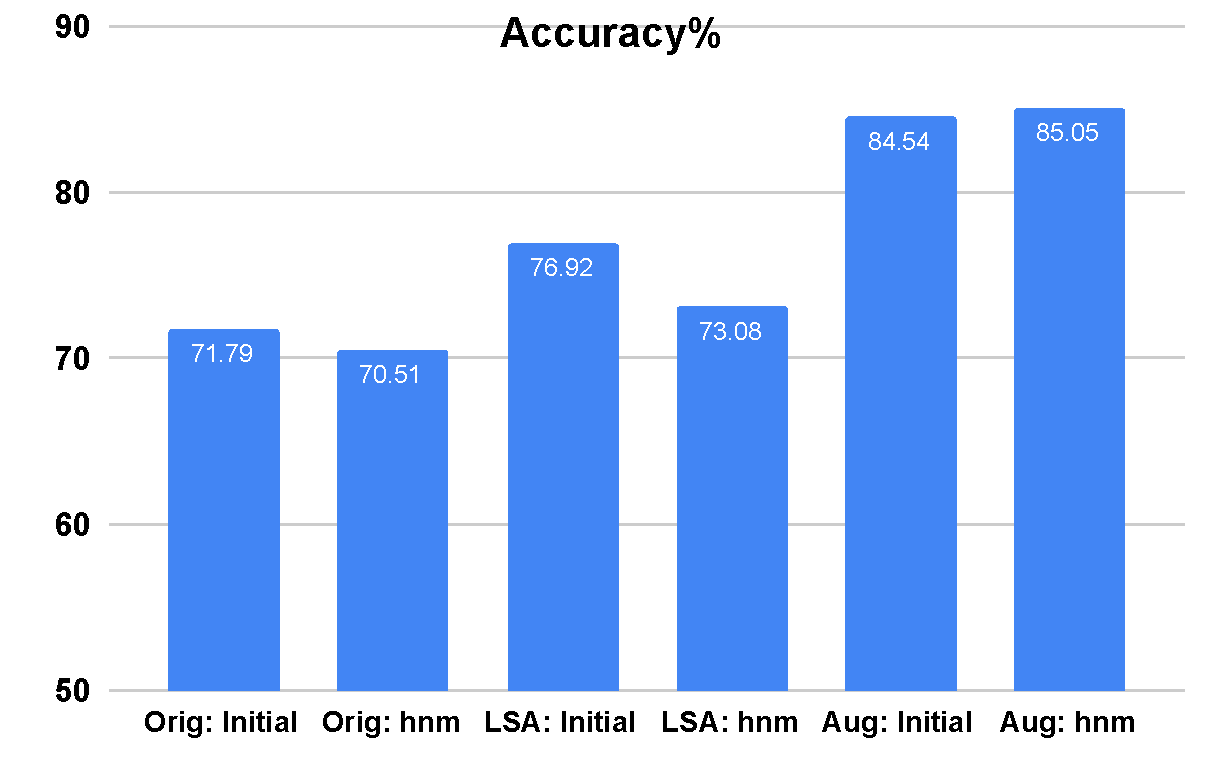
\includegraphics[scale=0.35]{Figs/chap4/vggacc.pdf}
          \caption{Accuracy}
     \end{subfigure}
     ~
     \begin{subfigure}[b]{0.5\linewidth}
         \centering
          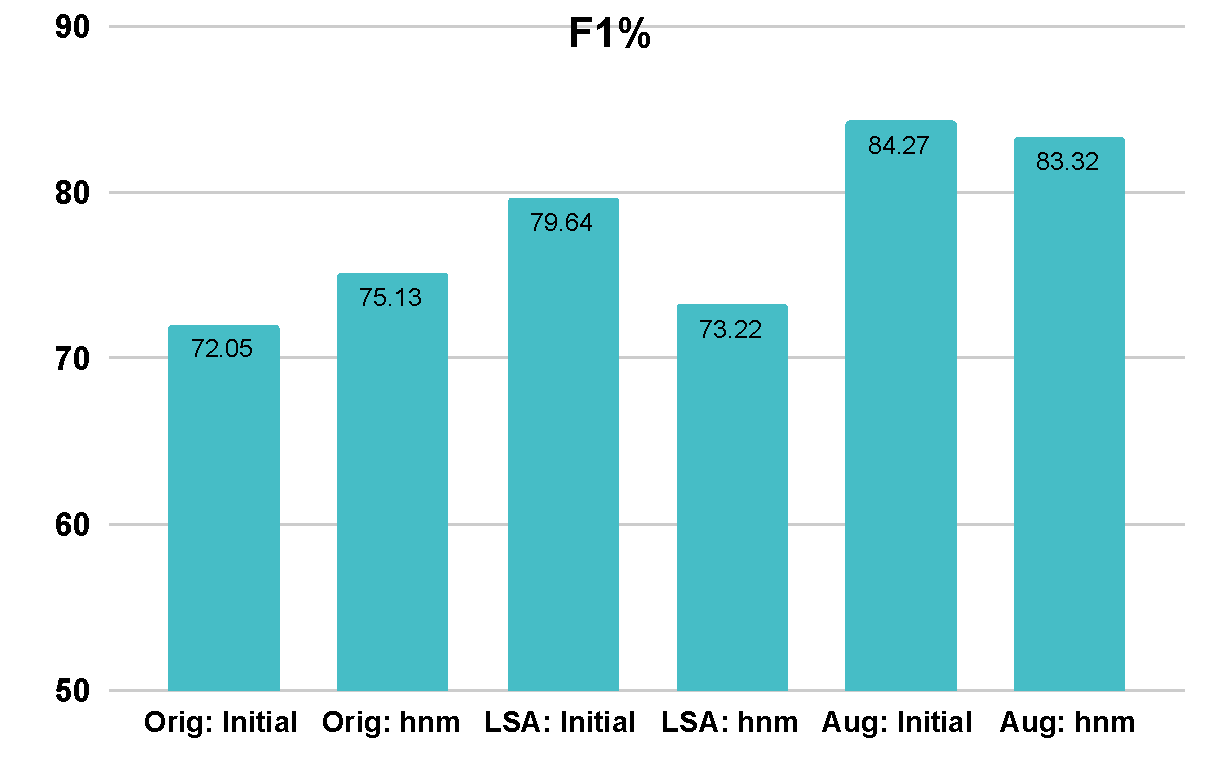
\includegraphics[scale=0.35]{Figs/chap4/vggf.pdf}
          \caption{F1 score}
     \end{subfigure}
     \\
     \begin{subfigure}[b]{0.5\linewidth}
         \centering
          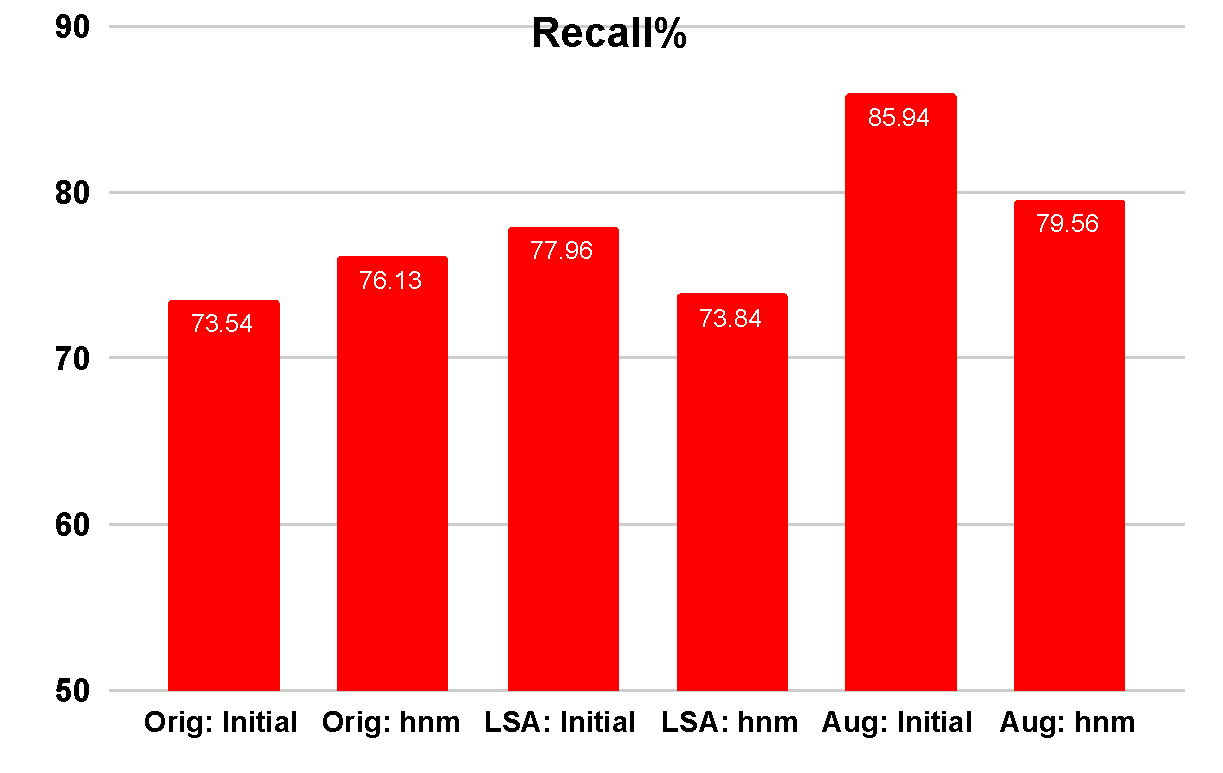
\includegraphics[scale=0.35]{Figs/chap4/vggrec.pdf}
          \caption{Recall}
     \end{subfigure}
     \begin{subfigure}[b]{0.5\linewidth}
         \centering
          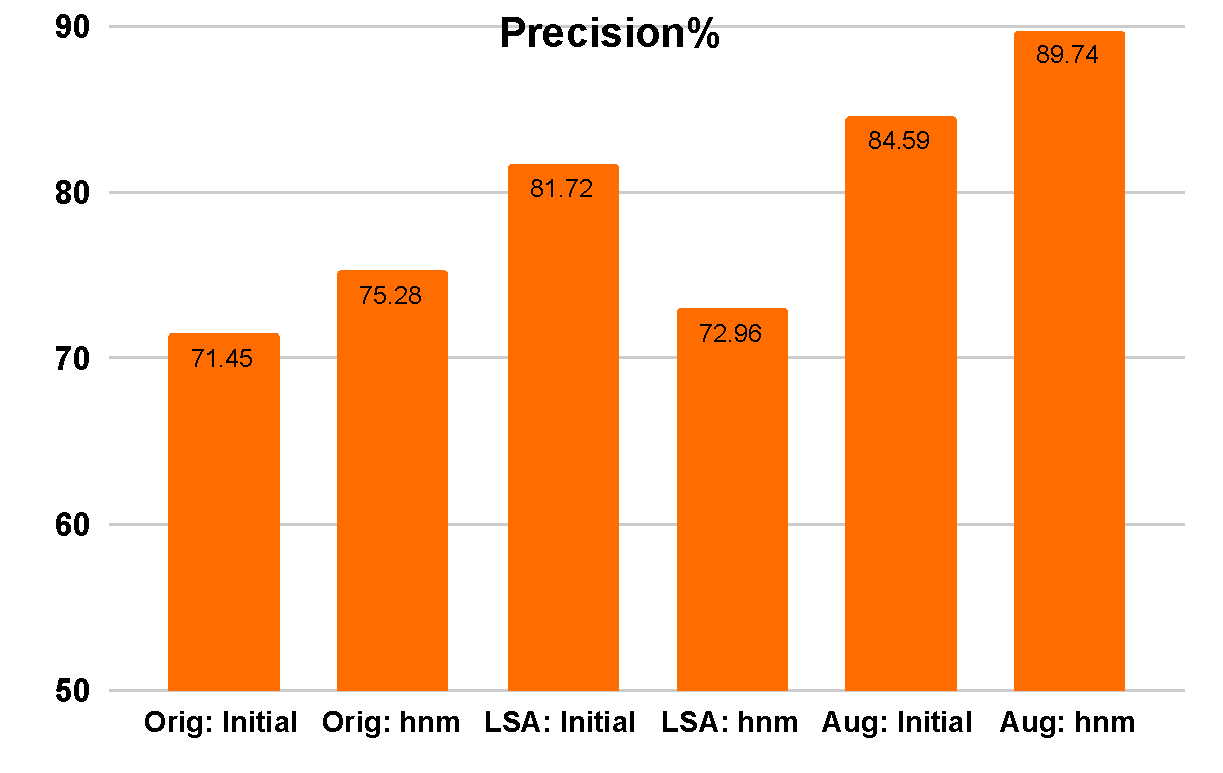
\includegraphics[scale=0.35]{Figs/chap4/vggpre.pdf}
          \caption{Precision}
     \end{subfigure}
  \caption{Histograms of VGG-based model: comparing 7 different strategies in accuracy, F1, recall and precision}
  \label{Fig:histvgg}
\end{figure}
\subsection{Position Detection on New Testing Data}
As illustrated previously, the metric scores were measured on fix dataset to evaluate the model performance. In order to compare the capability of generalisation among models, new test data were manipulated to examine the predictions of trained models. All audio files were clipped into 3-seconds segments, resulting in totally 4660 clips. Each clip records its clipped position in the raw audio file. Afterwards, the trained models are used to predict all clips and compare the actual position label in 'Praat' files. The prediction is considered as false positive if it not only was incorrectly classified but also has over 90\% confidence scores (the output of sigmoid in the last layer of network presenting in percentage). Table \ref{tab:wrong pos} shows the number of wrong predictions for trained models of all strategies. The less wrong predictions were detected, the higher capability of generalisation.\par
\begin{table}[htp]
    \centering
    \caption{Wrong predicted positions of two models}
    \label{tab:wrong pos}
    \resizebox{0.8\textwidth}{!}{%
    \begin{tabular}{|l|cc|cc|}
    \hline
     & \multicolumn{2}{c|}{Baseline} & \multicolumn{2}{c|}{VGG-based} \\ \cline{2-5} 
     & \multicolumn{1}{c|}{Num.} & Error\% & \multicolumn{1}{c|}{Num.} & Error\% \\ \hline
    Orig: Initial & 876 & 18.79 & 517 & 11.09 \\
    Orig: hnm & 748 & 16.05 & 421 & 9.03 \\ \hline
    LSA: Initial & 479 & 10.27 & 309 & 6.63 \\
    LSA: hnm & 455 & 9.76 & 280 & 6.01 \\ \hline
    Aug: Initial & 389 & 8.35 & 203 & 4.36 \\
    Aug: hnm & \textbf{353} &\textbf{7.58} & \textbf{157} & \textbf{3.37} \\ \hline
    \# average time (mins) & \multicolumn{2}{c|}{3.74} & \multicolumn{2}{c|}{32.36} \\ \hline
    \end{tabular}%
    }
\end{table}
In general, the incorrect number of prediction is descending with the order of strategies for both models. Using hard negatives to train model second time can optimize model to a certain extent. As to baseline, the MMSE-LSA shows outstanding scores with 84.41\% accuracy and 78.79\% F1 score in Table \ref{tabel:base dataset}, based on which this model was optimal. However, the number of wrong position for augmentation dataset is minimum, which means the generalisation error is lower than denoised dataset. There are two main reasons caused the higher generalisation error of denoised dataset. Firstly, the number of denoised training data is quite smaller than the augmentation, which is not enough to completely train the network. Furthermore, it will introduce classification bias only trained model with denoised positives. Sine pure speech signals are unavailable in most of realistic situations, this trained model has limited ability to detect positive calls. However, denoising is still helpful to classify negative examples.

As to VGG-based model, results demonstrate that it has powerful and effective performance on classification, with 3.37\% error for augmentation. Therefore, increasing the architecture depth of network can significantly enhance the ability of robustness and generalisation. Nevertheless, the main drawback for VGG-based model is time. Due to the increasing number of parameters and depth of network, both training and predicting are time-consuming efforts, compared with baseline model. It took 8.33 seconds on average for VGG-based model to predict one-minute long file, while baseline took less than 1 second.
However, it is still prominently efficient and effective than manually labelling. Although there were still amounts of wrong positions, all prediction results were recoded in file, which is beneficial to further manual check.
\section{Comparison of Optimal Models}
\begin{figure}[!htb]
     \begin{subfigure}[b]{0.5\linewidth}
         \centering
          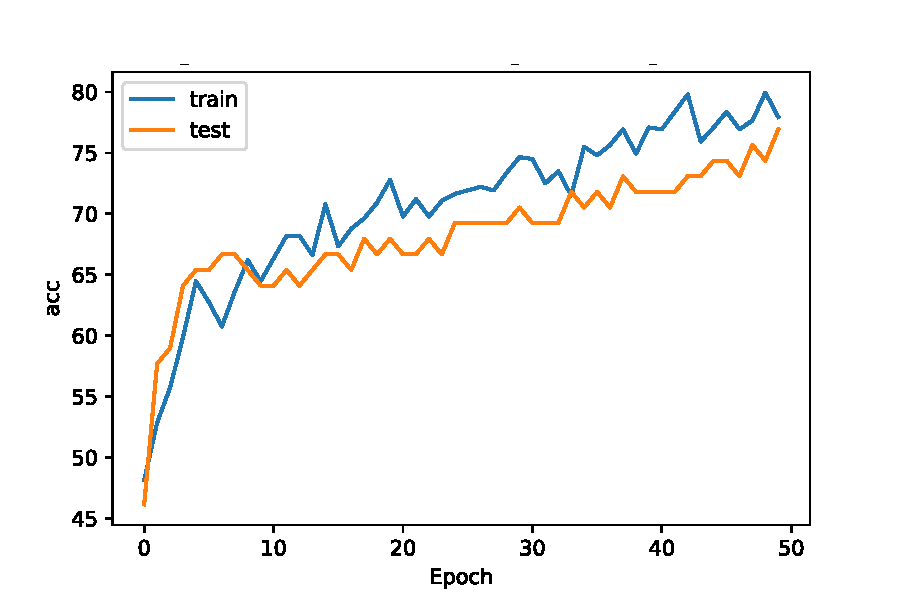
\includegraphics[scale=0.5]{Figs/chap4/denoised_e50_b16_acc.pdf}
          \caption{Baseline: accuracy }
     \end{subfigure}
     ~
     \begin{subfigure}[b]{0.5\linewidth}
         \centering
          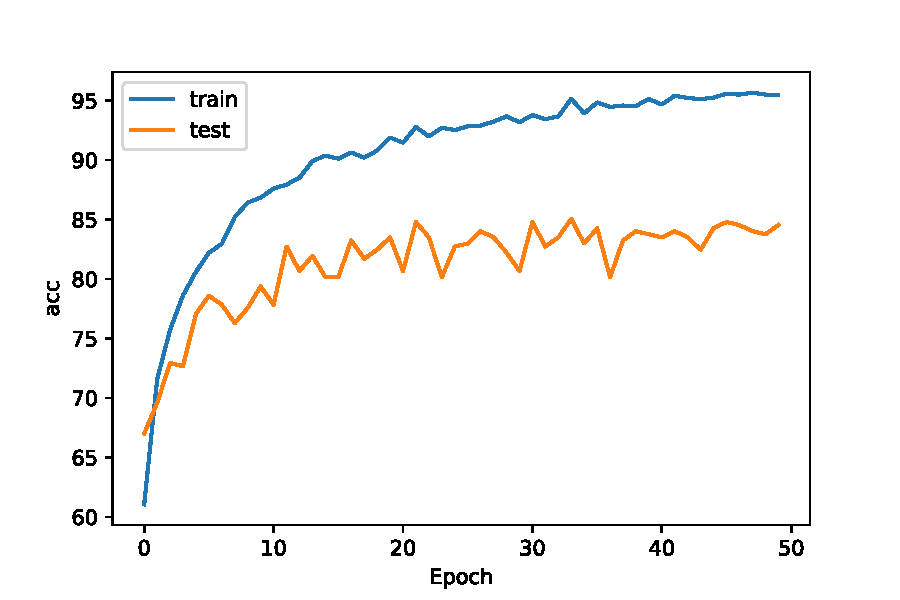
\includegraphics[scale=0.5]{Figs/chap4/vgg_augment_denoise_e50_b16_acc.pdf}
          \caption{VGG-based: accuracy }
     \end{subfigure}
     \\
     \vskip0.5em
     \begin{subfigure}[b]{0.5\linewidth}
         \centering
          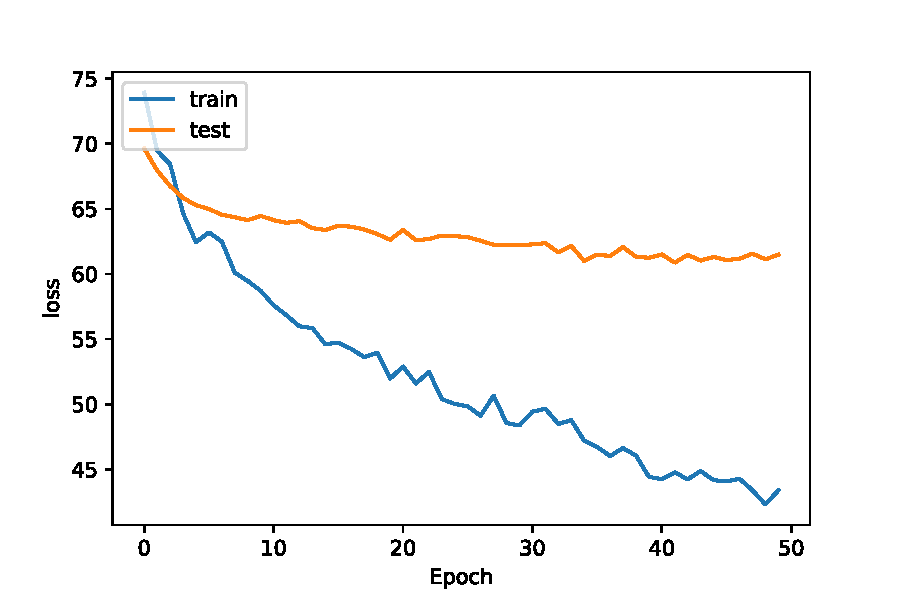
\includegraphics[scale=0.5]{Figs/chap4/denoised_e50_b16_loss.pdf}
          \caption{Baseline: loss}
     \end{subfigure}
     \begin{subfigure}[b]{0.5\linewidth}
         \centering
          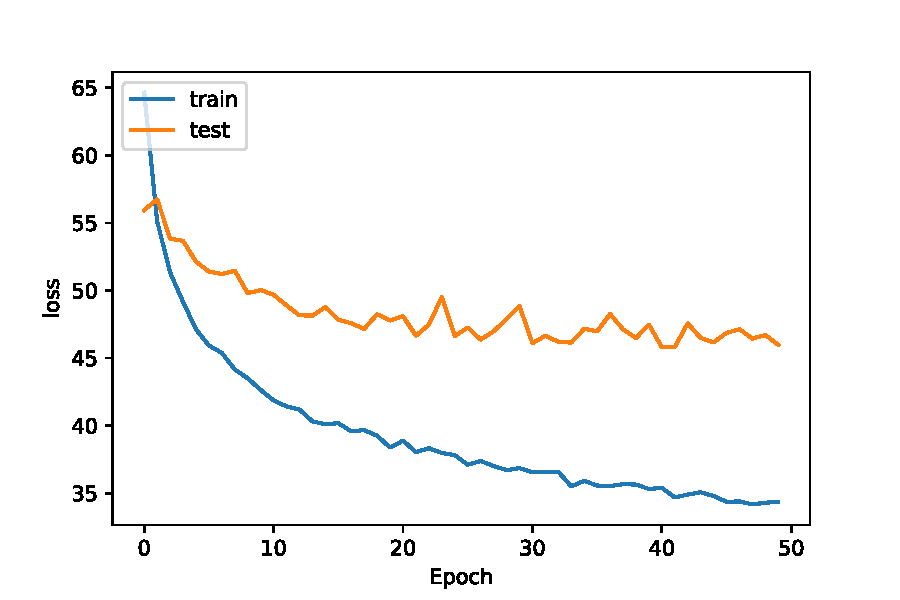
\includegraphics[scale=0.5]{Figs/chap4/vgg_augment_denoise_e50_b16_loss.pdf}
          \caption{VGG-based: loss}
     \end{subfigure}
  \caption{Accuracy and loss curves for optimal baseline (LSA: Initial) and VGG-based models (Aug: hnm) with epoch=50, batch\_size=16, lr=$10^{-5}$}
  \label{Fig:curve}
\end{figure}
Fig \ref{Fig:curve} depicts the accuracy and loss curves of two optimal model. The train and test accuracy have less difference for baseline model. Both of them gradually rise up and reach peak point with approximate 75\%. As to the VGG-based model, the training accuracy rapidly increases to 90\% at 15 epochs. Afterwards, both of accuracy curves gently increase until convergence. As a consequence, the test accuracy reaches 85.5\%, while the accuracy of training is up to 95\%. The test loss of denoised dataset for baseline model is difficult to reduce compared with VGG-based model. Thus, the gap between test and train loss is getting larger with increasing epochs. This may bring out the over-fitting problem with high generalisation error. However, the VGG-based model is significant robust and steady. The test loss can converge to approximately 0.45 after 50 epochs. Overall, the VGG-based architecture can effectively improve the classification performance, with relative outstanding metric scores and generalisation error.\par

Observing scores in Table \ref{tabel:base dataset} and Fig \ref{Fig:hist}, recall is generally lower than accuracy among all strategies. It means that certain positives are always classified as false negatives by baseline model, which indicates that there are a number of hard positive in the training dataset. Fig \ref{Fig:type} illustrates four types of positive and negative with easy and hard examples respectively. By comparing the difference of mel-spectrogram among examples, reasons for limited performance on positive data can be found. \par
\begin{figure}[!htb]
\hspace*{-2em}
     \begin{subfigure}[b]{0.5\textwidth}
         \centering
          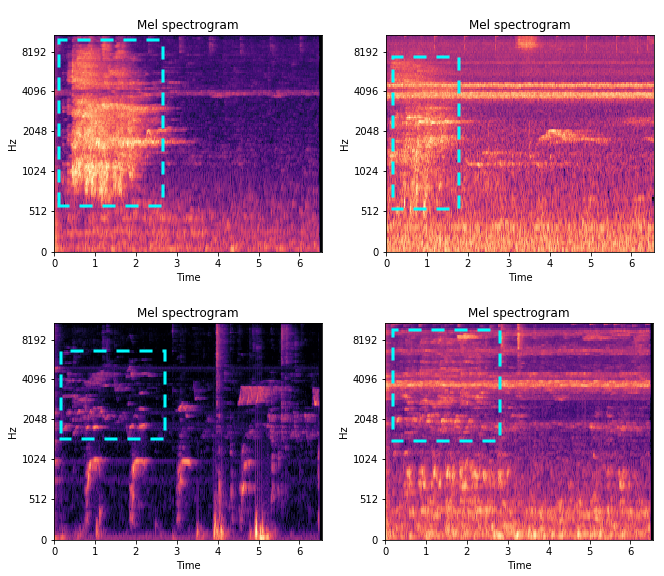
\includegraphics[scale=0.33]{Figs/chap4/pos.png}
          \caption{\centering Positive calls: Clear call (top\_left); Clear$+$Noise (top\_right); Unclear call (low\_left); Unclear$+$Noise (low\_right)}
     \end{subfigure}
     \hfill
     \begin{subfigure}[b]{0.5\textwidth}
         \centering
          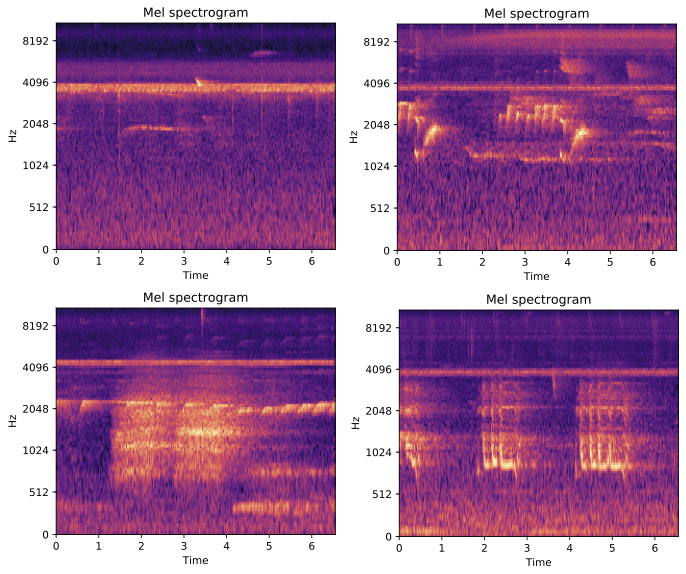
\includegraphics[scale=0.33]{Figs/chap4/neg.png}
          \caption{\centering Negative: Environmental noise (top\_left); Bird (top\_right); Howler monkey (low\_left); Macaws (low\_right)}
     \end{subfigure}
  \caption{Types of positives and negatives with easy and hard examples}
  \label{Fig:type}
\end{figure}
The quality of positives is relatively inconsistent during data collection. There are approximately four types of positives, namely clear calls (easy positives); clear calls covered by noise (relatively easy); unclear calls (relatively hard); unclear calls covered by noise (hardest). As to negatives, the environmental noise is the easy negative sample, while other animal calls (bird, Howler monkey and macaws et al.) increase difficulties on classification. Howler monkey calls have similar spectral characteristics in frequency and time. This similarity between negative spectrograms and hard positives confused the baseline model to a large extent. Hence, it is an arduous task for baseline to detect hard positives using low-level features, leading to lower recall than accuracy. After applying hard negative mining method, the distance of centres between negatives and positives tends to shrink, resulting in increased precision and decreased recall. Thus, hard positive mining can be applied as a further improvement. However, the VGG-based model slightly suffers from this issue, since high-level features can be extracted even from unclear calls. 


